\chapter{Planning system}
\label{ch:planning_system}
In this chapter the general framework adopted is discussed, proposing a suitable task planning system. After the  review of the current state of the art of task planners, a proper planner is chosen and then a suitable description to the table clearing problem is discussed.
\section{Task Planners Review}
To choose the proper planner for the task we evaluated three main categories of planners:
\begin{enumerate}
\item classical planners,
\item hierarchical planners,
\item probabilistic planners.
\end{enumerate}
\textbf{Classical planners} are characterized by environments which are fully observable, deterministic, finite and static (changes happen only when the agent acts) and discrete (in time, actions, objects...) \citep{artificialIntelligence}.  A very well known classic planner is the Fast Downward planner \cite{helmert2006fast}.


\textbf{Hierarchical planning}, also called \textit{Hierarchical Task Network}(HTN), works in a similar way to how it is believed that human planning 
works \citep{marthi2007angelic}. It is based on a reduction of the problem. The planner recursively decomposes tasks into subtasks, stopping when it reaches primitive tasks that can be performed directly by planning operators. This kind of planner needs to have a set of methods, where each method is a schema for decomposing a particular kind of task into a set of subtasks. For this kind of planning technique a well known planner is SHOP \citep{shop}.

\textbf{Probabilistic planning} is a planning technique which considers that the environment is not deterministic but probabilistic. So the actions have a probability to obtain a certain state, and given an initial and goal, the planner finds the solution path with the highest reward, which depends also on the probability. Probabilist problems are usually formalized as Markov Decision Processes (MDP).
%A probabilistic problem is generally formulated as a $6$-tuple $\Pi=\langle S, s_o, G, O, T, A \rangle$ %\cite{little2007probabilistic}, where:
%\begin{itemize}
%item $S$ is a finite set of states;
%\item $s_o \in S$ is the initial state;
%\item $G \in S$ is a goal state;
%\item $O$ is the set of outcomes, the probability of $o \in O$ is $Pr(o)$;
%\item $T(o,s) \in S$ is a (total) deterministic transition function for all outcomes $o \in O$ and states $s\in S$;
%\item $A(s)$ is a set of applicable actions for each $s %\in S$, coupled to a function $out(a) \subseteq O$ mapping each action to a set of outcomes in such a way that 
%\begin{itemize}
%\item each outcome $o \in O$ belongs exactly to one action $act(o)$;
%\item $\sum_{o \in out(a)} Pr(o) = 1$ for all $a$.
%\end{itemize}
%\end{itemize}
In this category two probabilistic planners that performed good in planning competitions are Gourmand \cite{Gourmand} and PROST \cite{PROST}.

\section{Planner}
%The problem this thesis is facing could be solved by several approaches by using planners from all the categories. We have already seen that such a problem involves geometric constraints and those cannot be considered directly by the planner using a ready to use state of the art planner, that would imply a designing of a new planner. Moreover using a hybrid planner is also time consuming, so we decided to focuse on a strategy that would let us to use already existing planners. This way involves working with symbolic predicates. Symbolic predicates are predicates which can be true or false, and they will be introduced more in detail in the next sections. 

The problem involves a big amount of uncertainty due to the interaction of the robot with the environment. When the robot interacts with the objects, it is very hard to predict correctly the position of the object after the execution, that is the next state. A probabilistic planner considers the probability associated with every effect to predict the state after executing an action, such a probability has to be specified or learned for each type of object.

Martinez et al. \citep{martinez2015planning} faced the problem of cleaning a surface entirely by probabilistic symbolic planning. The problem they solved was characterized by a strong uncertainty, and a unexpected effect of an action would require to replan and therefore to slow down the system.
Another way to face the problem of probability is replanning after each executed action \cite{kaelbling2012unifying}, or whenever the current state deviates from the expected one, generating a new plan from the current state to the goal. In this case the actions are considered deterministic, and only the first action is executed before replanning again. 

Little et al. discussed in \cite{little2007probabilistic} the problem of when is more useful the probabilistic planning with respect a simple replanning system. 
%They defined the concept of \textit{Probabilistic Interesting Problem} with the following definition:
%\begin{displayquote}
%A probabilistic planning problem is considered to be \textit{probabilistically interesting} if and only if it has all of the following structural properties:
%\begin{itemize}
%\item there are multiple goal trajectories;
%\item there is at least one pair of distinct goal trajectories, $\tau$
%and $\tau'$, that share a common sequence of outcomes for the first $n-1$ outcomes, and where $\tau_n$ and $\tau_n'$ are distinct outcomes of the same action; and
%\item there exist two distinct goal trajectories $\tau$ and $\tau'$ and outcomes $o \in \tau$ and $o' \in \tau'$ of two distinct actions $a = act(o)$ and $a' = act(o')$  such that executing action $a$ strictly decreases the maximum probability of reaching a state where action $a'$ can be executed. To clarify: executing $a$ rules out any plan with a maximal probability of executing $a'$.
%\end{itemize}
%\end{displayquote}
They defined a planning problem \textit{probabilistic interesting} if dead ends can be avoided,
exist multiple goal trajectories and there is at least one pair of distinct goal trajectories, $\tau$ and $\tau^{'}$ that share a common sequence of outcomes for the first $n-1$ outcomes, and where $\tau_{n}$ and $\tau_{n}^{'}$ are distinct outcomes of the same action. 
% COMMENT: The following is the old one
%They defined a planning problem \textit{probabilistic interesting} if dead ends can be avoided or when there exist several feasible solutions with low probability such that blended have a greater probability to reach the goal than another single trajectory with an higher probability.

They assert that unless a probabilistic planning problem satisfies all of the conditions to be \textit{probabilistic interesting} then it is inevitable that a well-written replanner will outperform a well-written probabilistic planner. Moreover the authors do not negate the possibility that a deterministic replanner could perform optimally even for probabilistically interesting planning problems. 

To conclude, in many problems it is more efficient to replan with a deterministic planner rather than directly using a probabilitic planner. 


Taking into account such considerations and that, except for rare cases, our planning problem is not \textit{probabilistic interesting}, the problem has been thought to be solved by a deterministic planner.

A hierarchical planner would be a good choice if the problem presented some hierarchies, for instance in the case the goal was to clear several tables. Since the problem is about cleaning a single table it is more straightforward to use a classical planner.

The planner chosen was the \textbf{Fast Downward} planner \citep{helmert2006fast}, a very well know classic one. 
This planner is feature-wise complete, stable and fast in solving planning problems.

\section{Symbolic Predicates}

\subsection{Formulation}
The problem is formulated as a $6$-tuple $\Pi=\langle S, s_o, G, A, T, c \rangle$, where:
\begin{itemize}
\item $S$ is a finite set of states;
\item $s_o \in S$ is an initial state;
\item $G \in S$ is a goal state;
\item $A(s)$ is a set of applicable actions for each $s \in S$;
\item $T(a,s) :$ $ S \times A \times S$ is a deterministic transition function;
\item $c(a)$ is the cost to apply action $a$.
\end{itemize}
The plans $\tau_i$ are sequences of actions applicable from the initial state until the goal state. The cost of a trajectory $C(\tau_i)$ is the sum of the cost of the actions of the trajectory $C(\tau_i) = \sum_{a \in \tau} c(a)$. The optimal solution is the solution with less cost: $\tau^* = \min_{\tau_i} c(\tau_i)$.
In this work we do not specify specific costs for the actions, so the planner returns the plan with fewer actions.


\subsection{Predicates}
The \textit{Fast Downward} planner needs the problem to be formulated in \textit{Problem Domain Description Language} (PDDL) \citep{pddl}. In this section the symbolic predicates that have been considered in order to solve the problem are described.

The task this thesis faces is a common task done by humans, who think in order to find a feasible sequence of actions. Such a sequence is normally composed of actions that avoid the collision between the manipulated objects and the other ones, whenever possible. To do this we, as humans, think on what is going to happen if we manipulate an object in a certain way. The design of the problem has been inspired by such a reasoning way and symbolic predicates are added so that the planner can reason about collisions and geometrical constraints.

As described in the introduction, the system will be able to perform two types of actions: \textbf{pushing} and \textbf{grasping}.
Grasping action is a necessary action in order to grasp an object and drop it into a bin, while the pushing action is an auxiliary action which has the aim to move an object in a pose that do not obstacle the solution of the problem. 
The pushing action is said to be auxiliary because it is not strictly necessary to solve every kind of problem, depending on the cluttered scene the grasping action could be enough.
The blending of these two actions makes wider the range of problem this planner can solve.    

The symbolic predicates are designed accordingly to the available actions trying to answer the following questions:
\begin{itemize}
\item When can an object be grasped? 
\item When can a object be pushed? In which direction? 
\end{itemize}
Answering these questions the following predicates are defined:

\begin{itemize}
\item \textbf{removed}: \ttt{(removed o1)} means that object \ttt{o1} has been grasped and dropped into the bin. The goal is reached when all the object have been removed. 
\item \textbf{on}:\ttt{(on o1 o2)} means that object \ttt{o1} stands on top of object \ttt{o2}. This predicate is defined since we don't want to interact with an object that has objects on top of itself. If we would grasp it, the object above would likely fall corrupting in this way the scene. That behaviour is undesired since a human would not grasp the bottom object without first grabbing the one on the top. Similarly for the pushing action, when an object with objects on top of itself is pushed, they could fall or collide with other objects. Vice versa if it was on top of other objects.
\item \textbf{block\_grasp}: \ttt{(block\_grasp o1 o2)} means that object \ttt{o1} obstacles  object \ttt{o2} to be grasped. 
Once we are sure that an object has no objects on top of it we have to check if it can be grasped, that is if the gripper will collide with object \ttt{o2} attempting to grasp the desired one. With this predicate the planner knows that the robot has first to interact with those objects before to grasp the desired one.
\item \textbf{block\_dir1}, \textbf{block\_dir2}, \textbf{block\_dir3}, \textbf{block\_dir4}: \ttt{(block\_dir1 o1 o2)} means that object \ttt{o1} obstacles  object \ttt{o2} to be moved along direction 1. We will consider 4 possible pushing directions (defined in Chapter \ref{ch:implementation}) per object. Being observant to the philosophy  of human-inspired actions, we avoid collisions when we push an object. To do so we translate the object along the pushing direction, for a certain length, and check for collision. Moreover, to push an object the end effector has to be put in the opposite side with respect the pushing direction, so an object cannot be pushed along a certain direction even in the case the gripper collides with an object.
Therefore if an object cannot be moved along a certain direction it is because the object would collide, or the gripper would collide.
\item \textbf{ik\_unfeasible\_dir1}, \textbf{ik\_unfeasible\_dir2}, \textbf{ik\_unfeasible\_dir3}, \textbf{ik\_unfeasible\_dir4}, \textbf{ik\_unfeasible\_grasp}: to consider the geometrical constraints regarding the working space of the robot, a predicate which states whether the inverse kinematic has solution is added for each action. For instance, \ttt{(ik\_unfeasible\_dir1 o1)} means that the inverse kinematic to push the object \ttt{o1} along direction 1 has no solution. %These predicates are added in order to consider the geometrical constraints regarding the working space of the robot.
\end{itemize}

\subsection{Actions}
In this section the actions preconditions and effects are described.

\paragraph{Grasping Action}
The \textbf{preconditions} to grasp a certain object are:
\begin{itemize}
\item no object stands on top of it,
\item no object collides with the gripper attempting to grab the desired object,
\item the inverse kinematic has solution.
\end{itemize}
The \textbf{effects} of the grasping action are:
\begin{itemize}
\item the grasped object is removed and dropped into the bin,
\item the grasped object no more blocks other object to be pushed or grasped,
\item if the grasped object was on top of other ones, it is no more on top of them.
\end{itemize}  

\paragraph{Pushing Action}
The \textbf{preconditions} to push a certain object, along a certain direction, are:
\begin{itemize}
\item no object stands on top of it,
\item the manipulated object is not on top of other objects,
\item no object collides with the manipulated one, or with the gripper, when pushed,
\item the inverse kinematic has solution.
\end{itemize}
In particular we defined 4 pushing action, one per pushing direction. 
The symbolic planner is not able to capture all the geometrical information of the problem through symbolic predicates, therefore it is not able to predict the future position of the manipulated object, and so the future states. This problem was handled by considering the object to be pushed far enough in such a way it is singulated from the other ones.  
Therefore the \textbf{effects} of this action are:
\begin{itemize}
\item the manipulated object no more blocks other objects to be pushed or grasped,
\item the other objects no more block the manipulated object to be pushed or grasped.
\end{itemize}  

%\paragraph{Effects of the actions}
%The effects of the action has to change the current predicates of the problem in order to update coherently the state. For the \textit{grasping} action whenever an object is grasped, since we are working in a deterministic scenario, the object is supposed to be grasped successfully and dropped in the bin. If such an object was on top of other ones, it was impeding some objects to be pushed in some direction or to be grasped those predicates have to be update coherently. Moreover to considered that the object is no more in the scene the predicate \textbf{grasped} is added. In particular \texttt{(grasped o1)} means that the object labelled as \texttt{o1} has been grasped and dropped into the bin, and therefore there is nothing more to do with it. The \textit{pushing} action, still thinking in a deterministic scenario, is supposed to be done in a manner that the object will be moved far enough from the others in such a way that it can be considered isolated. Considering it is isolated from the others, if it was blocking some objects to be pushed in a certain direction now it will not impedes them no more, and the same if an object impeded the current one, so the \texttt{block\_dir}$_i$ predicates are update, and the \texttt{block\_grasp} as well.  

	
\subsection{Backtracking}
%The proposed planner until now does not include any geometric information, such as whether the robot can actually perform a certain action. It may happens that the object is outside the working space of the robot and this makes it hard to interact with. In such a case the robot will have a plan but it is impossible its execution, this make the plan unfeasible. 

The geometrical constraints related to the inverse kinematic of the robot are computationally expensive. Moreover, as the reader will see in Chapter \ref{ch:implementation}, the actions are defined by more poses, so the inverse kinematic is even more expensive, usually it is a matter of $2$ or $3$ seconds per action. Computing it for each possible action (we have 5 actions in total, one grasping action and 4 pushing actions) for each object would make the computation of the predicates too expensive making the planning system quite slow. Usually the objects are inside the working space of the robot and the computation of the \ttt{ik\_unfeasible} predicates is usually unnecessary.

To overcome this we used the \textbf{backtracking} technique\citep{Bidot2015}. 
Backtracking is based on a two-fold strategy:
\begin{enumerate}
\item checking if the plan is feasible, 
\item if it is not, the state is updated with the new information and the system repeats from point 1 until a feasible plan is obtained.
\end{enumerate} 
%Backtracking is based on updating the initial state, used to get the current plan, considering the geometrical constraints, and plan again with the updated initial state obtaining in this way a different plan that could be feasible. The obtained plan will still be evaluated and backtracked until a feasible plan is obtained or there exists no plan.
Planning symbolically is very fast therefore replanning several times is not a problem. With this method the inverse kinematic will be solved only for the action we want to execute, the first one of the plan, and no time is wasted in computing the inverse kinematic for unnecessary actions. If executing the first plan's action is not possible the equivalent \ttt{ik\_unfeasible} predicate is updated. The pseudo algorithm to get a plan is shown in Algorithm \ref{alg:backtracking}.
%\DMcomment{Summarize this. Backtracking is that 1) after a plan is done, we check if it is feasible, 2) if not feasible, update state with updated information and repeat 1) - I don't see the need to summerize this}

\begin{algorithm}
\caption{Planning procedure with backtracking.\\
\textbf{Inputs:} initial state $s_{0}$ and goal state $G$. \\
\textbf{Outputs:} a feasible plan or not plan at all. }\label{alg:backtracking}
\begin{algorithmic}
\Procedure{GetPlan}{$s_{0}$,$G$}
\Repeat
  \State $plan \gets$ \textsc{GetFastDownwardPlan}($s_{0}$,$G$)
  \If{\textsc{$\neg$isPlanEmpty}($plan$)} 
  		\Return NULL 
  \EndIf
  \State $action\gets$ \textsc{GetFirstAction}($plan$)
  \State $success \gets$ \textsc{HasIKSolution}($action$) 
  \If{$\neg success$}
    \State $s_{0} \gets$ \textsc{UpdateInitialState}($action$) 
  \EndIf
\Until{$success$}
\Return $plan$
\EndProcedure
\end{algorithmic}
\end{algorithm}  

%This technique has been sued before to consider geometrical constraints when planning. This is a considerable limitation of symbolic planning but since they are typically very fast to execute, backtracking and replanning will not make them too much slower.


It is possible that an object cannot be grasped on a certain pose, because the inverse kinematic has no solution, but it can be moved in a new pose in which it can be grasped. Therefore the pushing actions also will include the effect that the object of interest will have a solution of the inverse kinematic in the new pose. This is usually a rare case but it might happen.  In the case the object is in a pose where it cannot be neither grasped or pushed because of the inverse kinematic, first the planner will return as a solution to grasp it, then it will replan and the solution will be to push it in one direction and grasp it, and so until no action can be executed and there exist no solution for the plan. 

\begin{figure}[tb]
\centering
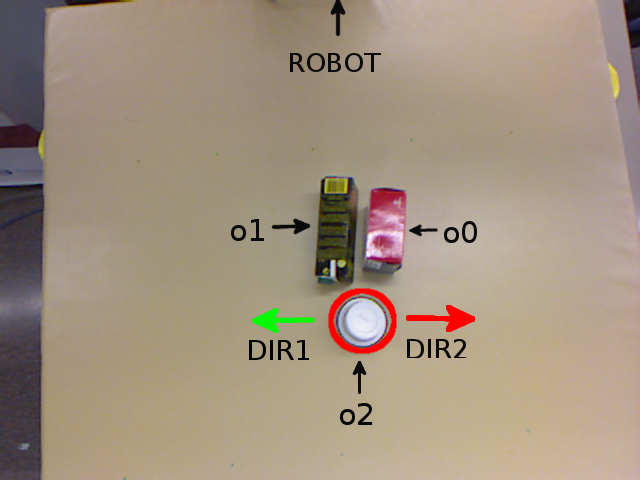
\includegraphics[width=6cm]{Img/backtracking/image4.png}
\caption{Unfeasible plan due to geometrical constraints. In this case the planner returns as action to execute grasping or pushing away the white cup (highlighted by a red circle) but it is out the configuration space of the robot and there exist no plan for that problem.} \label{fig:backtracking1}
\end{figure}

A situation in which the backtracking is useful is shown in Figure \ref{fig:backtracking1}. Accordingly to our strategy, the robot cannot grasp the black or red box because the gripper would collide, and the same for pushing them. It has to interact with the white cup in order to make space to move the other objects and then grasp them. For this case the system would perform the following set of operations:
\begin{enumerate}
\item It first gets the following plan: \texttt{(grasp o2)}, \texttt{(push\_dir1 o0)}, \texttt{(grasp o1)}, \texttt{(grasp o0)},

\item It solves the inverse kinematic for the \texttt{(grasp o2)} action, but it finds no solution and adds the predicate \ttt{(ik\_unfeasible\_grasp o2)}, 

\item It replans and gets the following plan: \texttt{(push\_dir1 o2)}, \texttt{(grasp o2)}, \texttt{(push\_dir1 o0)}, \texttt{(grasp o1)}, \texttt{(grasp o0)},

\item  It solves the inverse kinematic for the \texttt{(push\_dir1 o2)} action  but it finds no solution, so the predicate \ttt{(ik\_unfeasible\_dir1 o2)} is added,

\item It continues until there exists no solution for the planning problem.
\end{enumerate}

%The planner first returns the following plan: \texttt{(grasp o2)}, \texttt{(push\_dir1 o0)}, \texttt{(grasp o1)}, \texttt{(grasp o0)}. It tries to solve the inverse kinematic for the \texttt{(grasp o2)} action, but it finds no solution. Therefore the predicate \ttt{(ik\_unfeasible\_grasp o2)} is added and the planner replans. The new plan is: \texttt{(push\_dir1 o2)}, \texttt{(grasp o2)}, \texttt{(push\_dir1 o0)}, \texttt{(grasp o1)}, \texttt{(grasp o0)}. In this case it tries to get a solution for the inverse kinematic for the pushing action but it finds no solution, so the predicate \ttt{(ik\_unfeasible\_dir1 o2)} is added. And so on until the planner finds that all the possible actions for a feasible plan have no solutions for the inverse kinematic. In this way the planner includes the ability to understand also why no plan exists for a certain problem. \DMcomment{Itemize this in steps}

It may happen that the object outside the working space of the robot blocks the execution of the task because it is impossible to achieve the goal to grasp all the objects since one is outside the working space.
This happens when all the \ttt{ik\_unfeasible} predicates for an object are set to true. When this situation occurs the object is removed from the goals so that the rest of the goal can be completed.


It is important to point out again that the system is deterministic, meaning that all the actions are supposed to give the resultant state with a probability of $1$. Clearly the biggest uncertainty is related to the pushing action; the method used to select the pushing directions does not taken into account reliably the geometry of the object and the trajectory will be unlikely the desired one but a similar one. Overall the planner is considering to push the manipulated object at infinity to isolate it, and that's false. This is another uncertainty of the pushing action due to the lack of geometrical information.
 
After the execution of an action the planner gets a new depth image from the Kinect, it segments the scene, it recomputes the predicates and replans. In this way the planner considers a totally new problem and all the uncertainties associated to the previous plan will be solved by the current one. 
%In this manner we are forced to considered that some interactions between objects are allowed but tried to be avoid as much as possible. 

In order to provide a graphical scheme to the reader the perception and planning pipeline is depicted in Figure \ref{fig:pipeline}. It can be appreciated the two fold strategy of the algorithm, the first stage (Figure \ref{fig:pipeline1}) is devoted to get the predicates from the Kinect sensor and the second one to get a plan, to evaluate its feasibility and to execute it (Figure \ref{fig:pipeline2}).

\begin{figure}[tb]

\centering
\begin{subfigure}[t]{\textwidth}
\centering
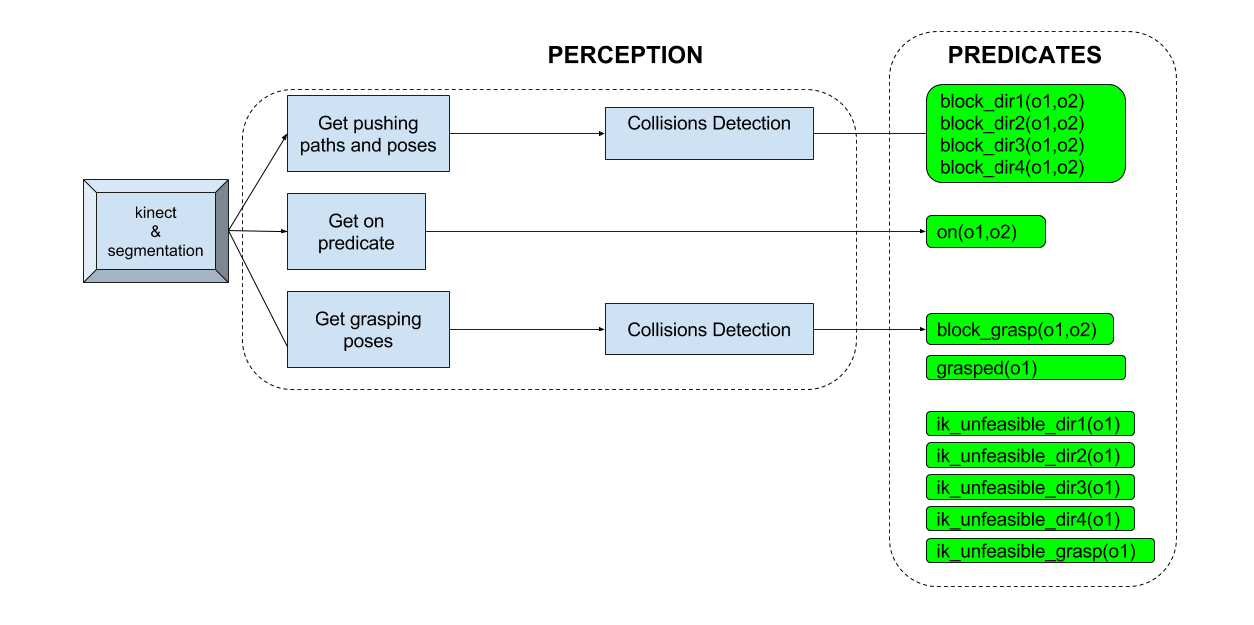
\includegraphics[width=\textwidth]{Img/planning/Pipeline1.png}
\caption{Perception Pipeline}\label{fig:pipeline1}
\end{subfigure}
\begin{subfigure}[t]{\textwidth}
\centering
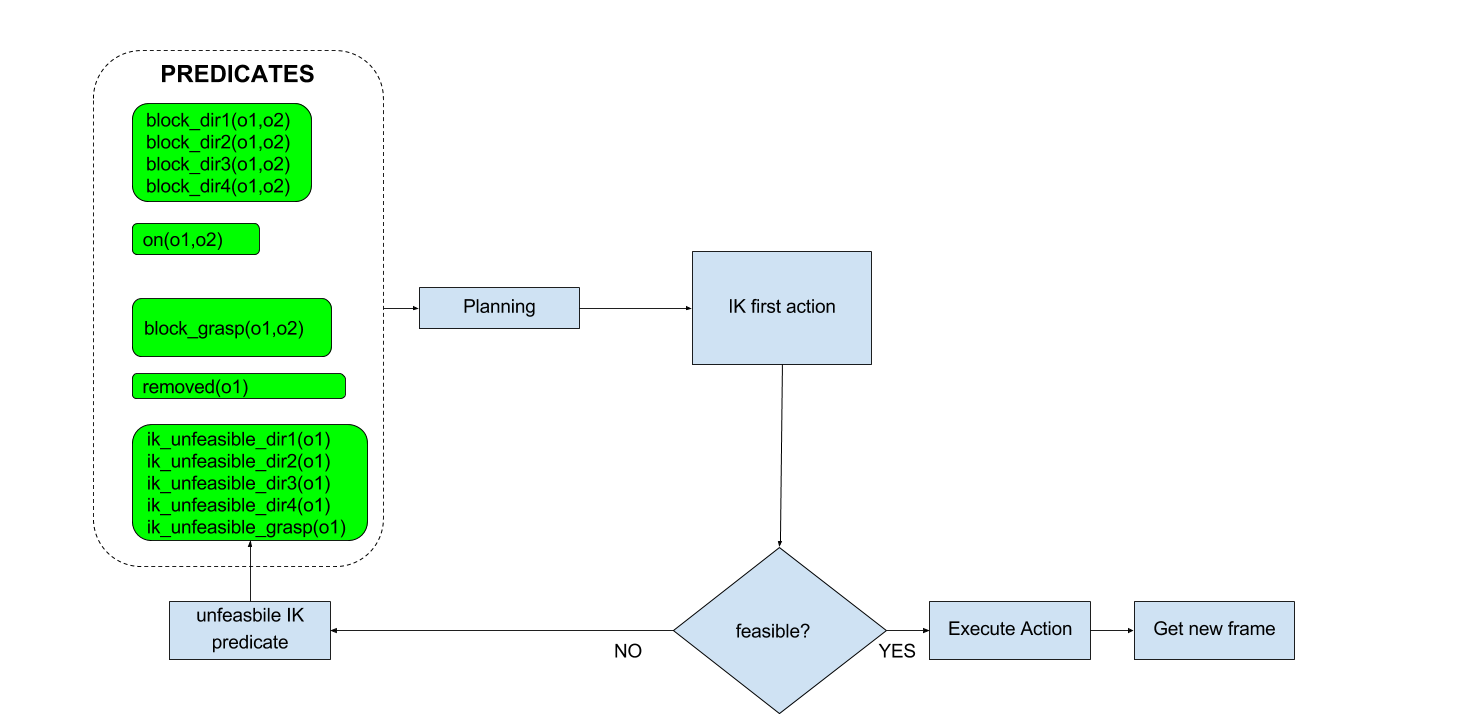
\includegraphics[width=\textwidth]{Img/planning/Pipeline2.png}
\caption{Planning Pipeline}\label{fig:pipeline2}
\end{subfigure}
\caption{Perception and planning pipeline}\label{fig:pipeline}
\end{figure}

\section{PDDL}
For clarity purposes, the PDDL syntax of the described actions is shown here. 
For the \textit{grasping} action its PDDL syntax is shown in listing \ref{graspPDDL}.

\lstset{language=pddl}
\begin{lstlisting}[caption={PDDL syntax of the grasping action},label=graspPDDL]
(:action grasp
    :parameters (?o - obj)
    :precondition (and
                  ; grasp it if the IK has a solution
                  (not (ik_unfeasible_grasp ?o))    
                  ; grasp it if there are no objects on its top
                  (not (exists (?x - obj)(on ?x ?o)))
                  ; grasp it if there is no object that blocks it
                  ; to be grasped
                  (not (exists (?x - obj)(block_grasp ?x ?o))))
    :effect (and
            ; the object "o" is removed
            (removed ?o)
            ; if the object was on top of other ones now it is
            ; no more on top of them
            (forall (?x - obj)
              (when (on ?o ?x)(not (on ?o ?x))))
            ; the grasped objects no more blocks other objects 
            ; to be pushed or grasped
            (forall (?x - obj)
              (and
              (when (block_grasp ?o ?x)(not (block_grasp ?o ?x)))
              (when (block_dir1 ?o ?x)(not (block_dir1 ?o ?x)))
              (when (block_dir2 ?o ?x)(not (block_dir2 ?o ?x)))
              (when (block_dir3 ?o ?x)(not (block_dir3 ?o ?x)))
              (when (block_dir4 ?o ?x)(not (block_dir4 ?o ?x))))
\end{lstlisting}

For the \textit{pushing} action its PDDL syntax is shown in listing \ref{pushPDDL}.

\lstset{language=pddl}
\begin{lstlisting}[caption={PDDL syntax of the pushing action along direction 1},label=pushPDDL]
(:action push_dir1
    :parameters (?o - obj)
    :precondition (and
                  ; push it if the IK has a solution
                  (not (ik_unfeasible_dir1 ?o)) 
                  ; push in direction 1 only if there are no
                  ; objects that block it along that direction
                  (not (exists (?x - obj)(block_dir1 ?x ?o)))
                  ; push it if it has no objects on top of it
                  ; and if it not on top of other ones
                  (not (exists (?x - obj)(on ?x ?o)))
                  (not (exists (?x - obj)(on ?o ?x))))
    :effect  (forall (?x - obj)
               (and
               ; once pushed the object is no more blocked in any direction
               ; and it no more blocks other objects to be moved
               (when (block_dir1 ?o ?x)(not (block_dir1 ?o ?x)))
               (when (block_dir2 ?o ?x)(not (block_dir2 ?o ?x)))
               (when (block_dir3 ?o ?x)(not (block_dir3 ?o ?x)))
               (when (block_dir4 ?o ?x)(not (block_dir4 ?o ?x)))
               (when (block_dir1 ?x ?o)(not (block_dir1 ?x ?o)))
               (when (block_dir2 ?x ?o)(not (block_dir2 ?x ?o)))
               (when (block_dir3 ?x ?o)(not (block_dir3 ?x ?o)))
               (when (block_dir4 ?x ?o)(not (block_dir4 ?x ?o)))
               ; once pushed it can be grasped and it no more
               ; blocks other objects to be grasped
               (when (block_grasp ?x ?o)(not (block_grasp ?x ?o)))
               (when (block_grasp ?o ?x)(not (block_grasp ?o ?x)))
               ; if before it cannot be grasped because of 
               ; the IK, we consider that the IK now has solution
               (when (ik_unfeasible_grasp ?o)(not (ik_unfeasible_grasp ?o))))))
\end{lstlisting}


%Notice that the \ttt{grasped} predicate is just a predicate used only by the planner in order to know when the object has been dropped into the bin or not, it does not need to be updated by the planning system. 





